\documentclass[twoside,12pt]{book}
\usepackage[utf8]{inputenc}
\usepackage[version=4]{mhchem} 
\newcommand\numberthis{\addtocounter{equation}{1}\tag{\theequation}}

\usepackage{titlesec}
\titleformat{\chapter}[display]   
{\normalfont\huge\bfseries}{\chaptertitlename\ \thechapter}{20pt}{\Huge}   
\titlespacing*{\chapter}{0pt}{-50pt}{40pt}

% Formatting of Figures
\usepackage{caption}
\usepackage{subcaption}
\usepackage{longtable}
\usepackage{chemfig}
\usepackage{siunitx}
\usepackage{graphicx}
\graphicspath{ {Figures/} }
\usepackage{wrapfig}
\usepackage{placeins}
\usepackage[capposition=top]{floatrow}
\usepackage{color}

% Bibliography
\usepackage[english]{babel}
\usepackage[backend=biber,style=numeric]{biblatex}
\addbibresource{ref.bib}

% ANN Figure
\usepackage{tikz}
\usetikzlibrary{arrows, automata, shapes, positioning}

% Formatting
\usepackage{setspace}
\doublespacing
\usepackage[a4paper,width=150mm,top=25mm,bottom=25mm,bindingoffset=6mm]{geometry}

\usepackage{titlesec}
\usepackage{fancyhdr}
\assignpagestyle{\chapter}{fancy}
\pagestyle{fancy}
\fancyhf{}
\fancyhead[LE,RO]{\thepage}
\renewcommand{\headrulewidth}{0pt} % remove lines as well
\renewcommand{\footrulewidth}{0pt}




\begin{document}

\frontmatter
\tableofcontents
\listoffigures
\listoftables

\chapter{Abstract}
Statistical data mining techniques, such as artificial neural networks (ANN), serve to address limitations of the current catalyst development and optimization approaches. Data mining techniques in conjunction with large catalytic data sets, should be able to assist in identifying meaningful materials descriptors, trends in catalytic reactivity and mechanistic differences between catalysts. This work explores the application of ANNs as sophisticated tools for identifying scaling relations using experimental low-temperature water-gas shift reaction data. We found that the ANN developed was capable of predicting catalytic activity for catalysts within the identified domain. Additionally, the ANN developed assisted in identifying catalysts which were not consistent with the ANN-optimized scaling relations.


\chapter{Acknowledgments}
I would like to take this opportunity to acknowledge those who have supported me through this scientific journey.\\
Prof. Dumesic and Prof. Huber, for providing the opportunity to work on this project, as well as intellectual and intuitive insight along the way.\\
WARF 2020 for financially supporting this project. \\
The educators and mentors who played a fundamental role in preparing me for a STEM career. Mrs. Jill Locke, who taught graphing using baby bunnies and never batted an eye at the many snakes and lizards I brought to her classroom. Dr. Susie Knetter for demonstrating how to wear the many hats of a successful scientist-friend-wife-mother. Prof. Detamore for introducing me to academic research and guiding me through the graduate school admission process. \\
The fellow scientists and friends who have been by my side for the past 18 months.\\
My parents, Paula \& Jeff Livingston, for being excellent role models and continually supporting my ambitious attitude and academic growth. From letting me be a turtle-catching, squirrel-raising little girl to driving me across town to participate in the IB Program to demonstrating curiosity and perseverance each day, they have contributed immeasurably to my successes. \\
My husband, Gehrig Keane, for always believing in me. 


\mainmatter


\chapter{Introduction}
\label{ch:intro}
%% -----------------------------------------------------------------------------
%% -----------------------------------------------------------------------------
\section{Motivations}
Statistical data mining techniques, such as artificial neural networks (ANN), serve to address limitations of the current catalyst development and optimization approaches (e.g., careful catalyst synthesis, characterization, and reactivity studies, combined with detailed density functional calculations). Data mining techniques in conjunction with large catalytic data sets, should be able to assist in identifying meaningful materials descriptors, trends in catalytic reactivity (scaling relations) and mechanistic differences between catalysts. This document details the exploration of these ideas for the water-gas shift (WGS) reaction (i.e., \ce{CO + H2O <--> CO2 + H2}).
%% -----------------------------------------------------------------------------
%% -----------------------------------------------------------------------------
\section{Machine Learning Fundamentals}
Data mining, the process of identifying patterns in large datasets, is a subfield of computer science at the intersection of statistics and machine learning (ML). Data mining algorithms enable computers to make predictions for complex, highly dimensional problems based on previously-encountered data. This project employs the use of artificial neural networks (ANN). ANNs are similar to traditional curve-fitting tools, which define an input-output relationship. However, ANNs differ from traditional curve-fitting models in their ability to fit highly dimensional datasets, such as those encountered in the field of catalysis. 

When developing an ANN, the model must first be `trained' using a set of examples referred to as `training data'. The training algorithm optimizes the model using training data to tune the model's mathematical parameters. While ANNs are frequently considered `black boxes', they actually consist of complex, statistically optimized mathematical functions. Trained with an appropriate data set, ANNs can be used to predict an optimum solution to a mathematically described problem. 

To place this work in the larger context of ML, the ANNs discussed in this document are a form of `supervised' ML. Each example or `instance' in the training data set consists of input information (a vector) and corresponding output information. This training data is considered `labeled' because each input instance is `labeled' with a corresponding output.

Architecturally, ANNs are similar to biological neural networks, storing and transferring information with numerical values rather than electrical impulses. Similar to a biological neural network, an ANN consists of many inter-connected `neurons' or `perceptrons', such as the one in figure \ref{fig:neuron}. For `feed-forward' networks, each neuron receives input signals from the preceding layer and sends an output signal to each neuron in the following layer \cite{Jacobson_2013}. 
	\begin{figure}[ht]
	    \centering
	    \includegraphics[width=0.6\textwidth]{Introduction/Neuron.png}
	    \caption{Example of an artificial neuron}
	    \label{fig:neuron}
	\end{figure}
Each input signal has an independent value. These input values are summed and then transformed by an `activation function' to produce a single output signal. Activation functions are typically step, linear or sigmoid functions. Mathematically, a neuron's output is determined by the activation function applied to the summation of the weighted inputs, shown in equations \ref{eq: input} and \ref{eq: output}.
	\begin{equation}
		input = w_1 x_1 + w_2 x_2 + \ldots + w_n x_n = \sum w_i x_i
		\label{eq: input} \end{equation}
	\begin{equation}
		output = f(input) = f\left( \sum w_i x_i \right)
		\label{eq: output} \end{equation}

When these neurons are linked together into a network, shown in figure \ref{fig:ANN}, the mathematical model becomes a complex function of weighted summations and activation functions. While many types of neural networks exist (i.e., deep, convolutional, relational, etc.) this report focuses on feed-forward neural networks with one or two layers of hidden neurons. Furthermore, information only travels in a forward-direction, there is no recursion or feedback within the network. The networks explored in this thesis only have a single output neuron.
	\begin{figure}[ht]
	    \centering
	    
	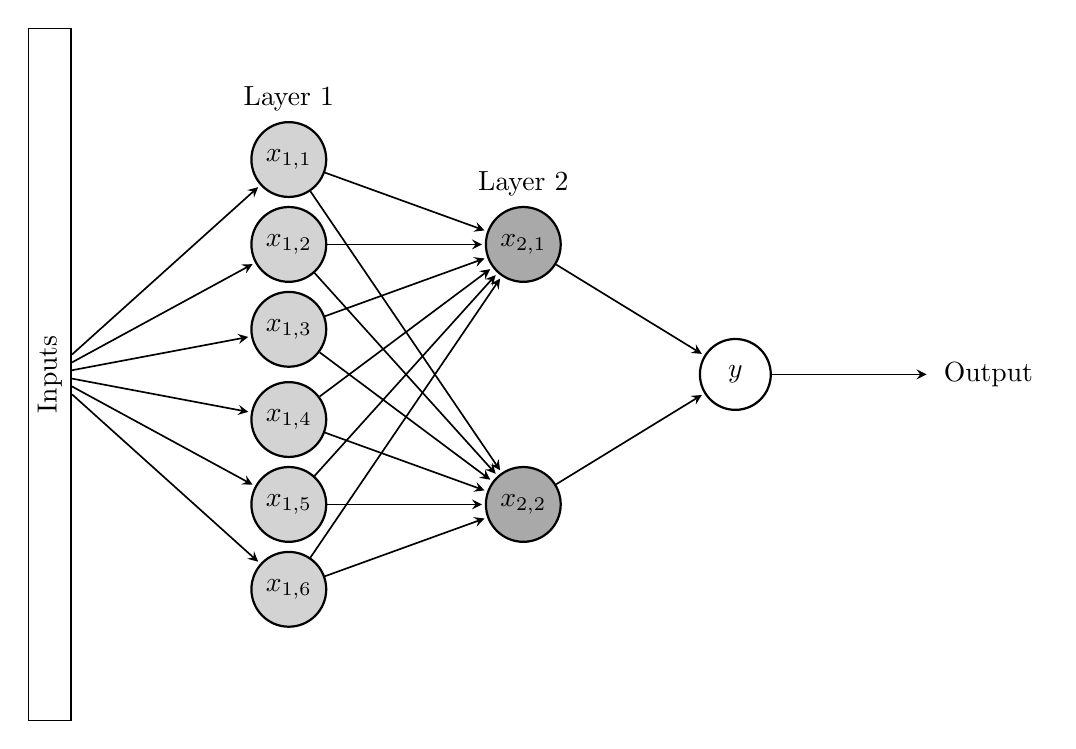
\begin{tikzpicture}[
			> = stealth, % arrow head style
			shorten > = 1pt, % don't touch arrow head to node
			auto,
			align=center,
			semithick, % line style
			node distance = 1mm and 2cm
		][h]

		\definecolor{awesome-grey}{RGB}{211,211,211}
		\definecolor{fantastic-grey}{RGB}{169,169,169}

		\tikzstyle{every state}=[draw = black, thick, fill = white, minimum size = 9mm]
		\tikzstyle{layer1}=[state,fill = awesome-grey]
		\tikzstyle{layer2}=[state,fill = fantastic-grey]
		\tikzstyle{invisible-border}=[state, draw = white, fill = white, minimum size = 1mm]
		\tikzstyle{inputs}=[rectangle, draw, text centered, minimum width=1.5em, minimum height=25em]%rotate around={90:(0,0)}

		% Input node is the root node positionally
		\node[inputs] (inputs) {\rotatebox{90}{Inputs}};

	% ----------------------------------------------------------------------
	% Layer 1
	% ----------------------------------------------------------------------
		% This node hides in between the Input box and layer 1 nodes for correct spacing...
		\node[invisible-border, right=0cm and 1mm of inputs] (spacing-anchor) {};

		% Nodes {x_11,x_12,x_13} are above right invisible-border
		\node[layer1, above right= of spacing-anchor] (x13) {$x_{1,3}$};
		\node[layer1, above= of x13] (x12) {$x_{1,2}$};
		\node[layer1, above= of x12, label=above:Layer 1] (x11) {$x_{1,1}$};

		% Nodes {x_14,x_15,x_16} are below invisible-border
		\node[layer1, below right= of spacing-anchor] (x14) {$x_{1,4}$};
		\node[layer1, below= of x14] (x15) {$x_{1,5}$};
		\node[layer1, below= of x15] (x16) {$x_{1,6}$};

		% Edges from input box -> {x_11,x_12,x_13,x_14,x_15,x_16}
		\path[->] (inputs) edge node {} (x11);
		\path[->] (inputs) edge node {} (x12);
		\path[->] (inputs) edge node {} (x13);
		\path[->] (inputs) edge node {} (x14);
		\path[->] (inputs) edge node {} (x15);
		\path[->] (inputs) edge node {} (x16);

	% ----------------------------------------------------------------------
	% Layer 2
	% ----------------------------------------------------------------------
		% Nodes {x_21,x_22} are above and below respectively
		\node[layer2, right= of x12, label=above:Layer 2] (x21) {$x_{2,1}$};
		\node[layer2, right= of x15] (x22) {$x_{2,2}$};

		% Edges from {x_11,x_12,x_13,x_14,x_15,x_16} -> {x_21,x_22}
		\path[->] (x11) edge node {} (x21);
		\path[->] (x11) edge node {} (x22);
		\path[->] (x12) edge node {} (x21);
		\path[->] (x12) edge node {} (x22);
		\path[->] (x13) edge node {} (x21);
		\path[->] (x13) edge node {} (x22);
		\path[->] (x14) edge node {} (x21);
		\path[->] (x14) edge node {} (x22);
		\path[->] (x15) edge node {} (x21);
		\path[->] (x15) edge node {} (x22);
		\path[->] (x16) edge node {} (x21);
		\path[->] (x16) edge node {} (x22);

	% ----------------------------------------------------------------------
	% Layer 3
	% ----------------------------------------------------------------------
		% Y and output
		\node[state, right=0cm and 7.5cm of spacing-anchor] (y) {$y$};
		\node[invisible-border, right= of y] (o) {Output};

		\path[->] (x21) edge node {} (y);
		\path[->] (x22) edge node {} (y);
		\path[->] (y) edge node {} (o);

	\end{tikzpicture}
        \caption{Simple feed-forward artificial neural network}
		\label{fig:ANN}
		\end{figure}

Consider the case with two hidden layers and a single output where the first hidden layer contains six neurons and the second layer contains two neurons, demonstrated in figure \ref{fig:ANN}.  Note that each of the neurons has the properties shown in figure \ref{fig:neuron}. To illustrate the mathematics contained in the `black box', begin by considering the output, $y$ as a function of the neurons $x_{2,1}$ and $x_{2,2}$ and their associated weights in the preceding layer, equation \ref{eq:output}. Similarly, the output from the $x_{2,1}$ and $x_{2,2}$  neurons is determined by the neurons in first hidden layer ($x_{1,1}$, $x_{1,2}$, $x_{1,3}$, $x_{1,4}$, $x_{1,5}$, $x_{1,6}$). The mathematical relationship between the first and second hidden layers is demonstrated in equations \ref{eq:x_2,1} and \ref{eq:x_2,2}. Finally, the output for each neuron in the first layer is given as a function of the network inputs ($in_1$ to $in_n$), equation \ref{eq:x_1,i}. 
		\begin{equation}
			y = f(x_{2,1}, x_{2,2}) 
			\label{eq:output}\end{equation}
		\begin{equation}
			x_{2,1} = f_{2,1}(x_{1,1}, x_{1,2}, x_{1,3}, x_{1,4}, x_{1,5}, x_{1,6}) 
			\label{eq:x_2,1}\end{equation}
		\begin{equation}
			x_{2,2} = f_{2,2}(x_{1,1}, x_{1,2}, x_{1,3}, x_{1,4}, x_{1,5}, x_{1,6})
			\label{eq:x_2,2}\end{equation}
		\begin{equation}
			x_{1,i} = f_{1,i}(in_1, in_2, \ldots, in_n)
			\label{eq:x_1,i}\end{equation}
To determine the overall function representing the ANN shown, begin by nesting the input-output functions for each layer. First, replace the $x_{2,1}$ and $x_{2,2}$ inputs in equation \ref{eq:output} with equations \ref{eq:x_2,1} and \ref{eq:x_2,2} to yield equation \ref{eq:output nested}. Then replacing the $x_{1,i}$ inputs in equation \ref{eq:output nested} with their corresponding equation \ref{eq:x_1,i} form yields the overall ANN representation in equation \ref{eq: output nested2}.
		\begin{equation}
			\begin{split}
			y = f\big[
				f_{2,1}(x_{1,1}, x_{1,2}, \ldots, x_{1,6}), \\
				f_{2,2}(x_{1,1}, x_{1,2}, \ldots, x_{1,6}) \big]
			\end{split}
			\label{eq:output nested}
			\end{equation}
		\begin{align*}
		y = f\big[
			f_{2,1} \big(
				&f_{1,1}(in_1, in_2, \ldots, in_n) \\
				&f_{1,2}(in_1, in_2, \ldots, in_n), \\
				& \ldots,\\
				&f_{1,6}(in_1, in_2, \ldots, in_n) ],\\
			f_{2,2} [
				&f_{1,1}(in_1, in_2, \ldots, in_n) \\
				&f_{1,2}(in_1, in_2, \ldots, in_n), \\
				& \ldots,\\
				&f_{1,6}(in_1, in_2, \ldots, in_n) \big)  \big] \numberthis
			\label{eq: output nested2}
			\end{align*}

In general, increasing the size of the training data set improves predictions. A common heuristic for determining the minimum size of the training data set is that there should be twice as many instances, or total data points, in the training data set as weights in the ANN \cite{Jacobson_2013}. For the most general feedforward ANN, the number of weights is determined by equation \ref{eq:num of weights}. For ANNs discussed in this work with two hidden layers and a single output, the number of weights is given by \ref{eq:specific num of weights}.
	\begin{equation}
		weights = n_{inputs}*n_{Layer1} + n_{Layer1}*n_{Layer2} + \ldots + n_{LastLayer}*n_{outputs}
		\label{eq:num of weights} \end{equation}
	\begin{equation}
		weights = n_{inputs}*n_{Layer1} + n_{Layer1}*n_{Layer2} + n_{Layer2}
		\label{eq:specific num of weights} \end{equation}
%% ----------------------------------------------------------------------------
%% -----------------------------------------------------------------------------
\section{Previous Work in Machine Learning \& \\Catalysis}
ML was initially proposed in the 1950's with backpropagation methods incorporated in 1986 \cite{Turing_1950,Rumelhart_1986}. Three years later, in 1989, Shigeharu Kito \& Tadashi Hattori pioneered ML as a tool for catalyst optimization \cite{Kito_1989}. ANNs have since been explored for optimizing materials/catalyst properties and reaction conditions as well as approximating computationally intensive calculations \cite{Omata_2004,Corma_2002,Kito_2004,Ulissi_2017}. As experimental techniques, ML methods and computational power advance, new and exciting opportunities to merge these fields develop.

	% -------------------------------------
	\subsection{Experimental Catalysis}
	The earliest and most-explored application of ML in catalysis has been in using ANNs to approximate the reactivity or selectivity for differing catalyst compositions. This movement was led by Kito \& Hattori who, in 1989, proposed INCAP (INtegration of Catalyst Activity Patterns), a system they claimed was capable of predicting the reaction mechanism, important catalytic functions, plausible side reactions, unfavorable products resulting from said side reactions and proposing catalyst candidates \cite{Kito_1989}. Kito \& Hattori continued publishing on ML in catalysis through 2006 \cite{Kito_2006}. Using ANNs they developed models to predict the acid strength of mixed oxides, predict the product selectivity for the oxidative dehydrogenation of methane, predict the catalyst deactivation in methanol conversion, and identify factors controlling catalytic activity \cite{Kito_1991,Kito_1994,Kito_2004,Kito_2006}. 

	Kohji Omata \& Muneyoshi Yamada also made significant contributions to the intersection of catalysis and ML. Together they published a series of papers exploring Radial Basis Function Networks (RBFN), which are similar to ANNs, for catalyst optimization. These networks optimized Co loading and preparation \cite{Omata_2006_1}, promoter optimization for oxidation of \ce{CO} and dry reforming of methane \cite{Omata_2009,Omata_2007,Omata_2010}. They also developed RBFNs for optimizing the preparation and composition of a Cu-Zn-Al-Sc-B-Zr catalyst for methanol synthesis, ternary-oxide Cu catalysts for steam reforming of methanol and promoters for \ce{Ni}/activated carbon catalysts for carbonylation of methanol \cite{Omata_2004,Omata_2004_2,Omata_2008}. Finally, Omata \& Yamada used RBFNs to optimize a Cu-Zn catalyst for dimethyl ether synthesis and a ZSM-5 catalyst for dimethyl ether to olefin conversion \cite{Omata_2006_2,Omata_2009_2}. For each application, their training data was largely generated `in house' using high throughput techniques. As attributes, Omata \& Yamada repeatedly chose to use chemical properties (molecular weight, boiling point, etc). However, he did not perform any analysis or optimization on the attributes chosen. 

	Finally, Avelino Corma has published on several diverse catalytic applications for ANNs and proposed a Design of Experiments framework. Corma began using ANNs to predict catalyst activity and selectivity for oxidative dehydrogenation of ethane \cite{Corma_2002}. The developed ANN used molar catalyst composition to predict reactant conversion, product yield and overall selectivity. More recently, Corma  et al. used ANNs with high throughput experimental techniques to optimize a \ce{Ti} catalyst for olefin epoxidation \cite{Corma_2005}. Additionally, they looked at ANNs and decision trees to successfully predict material properties (e.g., stability) based on composition for the high temperature synthesis of zeolites \cite{Corma_2006}. Finally, Corma et al. describe a `soft-computing framework' which combines a genetic algorithm, an ANN and high-throughput experimentation to rapidly optimize a catalyst within the defined domain \cite{Corma_2008}. Additionally, Corma has demonstrated the use of ANNs to optimize not only catalyst composition, but also reaction conditions and scale-up approaches, focusing on n-paraffin isomerization \cite{Corma_2003_1,Corma_2003_2}. 

	\subsection{Scaling Relations}

	In catalysis, scaling relations have been successfully used to drive development of novel catalytic materials and predict catalytic activity \cite{Greeley_2016}. Defining a scaling relation as any relationship in which a change to one variable causes a predictable and defined change in another variable and revisiting equations \ref{eq: output} through \ref{eq: output nested2}, it is clear that ANNs can be framed as a sophisticated scaling relationship tool. While each neuron alone performs a predictable transformation on its inputs, the network as a whole also fits within the definition of a scaling relationship. 

	Currently, scaling relations for heterogeneous catalysis relate elementary step activation energies to adsorption energies and thus reactivity of key intermediates \cite{Gani_2017}. However, it is well understood that catalysts cannot demonstrate activities above the peak of the volcano plot while obeying scaling relations \cite{Andersen_2017}. Therefore, identifying materials which break scaling relations may have important implications for future catalyst development. 
	
	% -------------------------------------
	\subsection{Explored in this Work}
	This work expands on the foundational work presented by increasing the catalyst domain space, incorporating diverse training data, optimizing attribute selection and incorporating DFT-derived descriptors. The laborious effort of Odabasi, Gunay and Yildrim resulted in a database of 4,360 data points for the water-gas shift (WGS) reaction derived from publications spanning 10 years (2002 to 2012) \cite{Odabasi_2014}. The data used for this work follows from the database constructed and published by Odabasi, Gunay and Yildrim. 

	Unlike the previous ANN studies cited, which largely rely on high-throughput data from individual research groups, the data in this study was collected in numerous laboratories with diverse experimental equipment and procedures. While much of the cited literature considers only a narrow scope of catalysts (i.e., only varying a single parameter such as promoter or active metal), this thesis considers many different supports, active metals, promoters, synthesis techniques and reactor conditions. To my knowledge, this is the first study using ANNs to combine DFT attributes (binding energies) with chemical properties to predict the fundamentally-explained forward rate. Furthermore, this works begins discussion on applying ML to derive scaling relations and evaluate meaningful catalyst attributes.  

\chapter{Methods}
\label{ch:methods}


%% -----------------------------------------------------------------------------
%% -----------------------------------------------------------------------------
\section{Original Dataset} 

A database of WGS reaction data was assembled and provided as Supplementary Materials by Odabasi et al. \cite{Odabasi_2014}. This data set is composed of 4,360 data points from 97 publications between 2002 and 2012. The Odabasi et al. explored trends in this data using data mining techniques including decision trees, ANNs and support vector machines. The data was organized and described categorically by support, primary metal and promoter metal attributes. The optimized NN, trained with MATLAB's neural network toolbox, predicted CO conversion. They report a training performance of $R^2$=0.972, MSE = 5.42 and a testing performance of $R^2$=0.905, MSE = 10.05 \cite{Odabasi_2014}. 

%% -----------------------------------------------------------------------------
%% -----------------------------------------------------------------------------
\section{Data Disqualification}
This study expands on the results of Odabasi et al. by developing an ANN with new attributes and outputs. Prior to ANN development, the original data was `cleaned' to remove data that did not align with the objectives of this project or the constraints defined. This process reduced the training data set from 4,360 instances to 1,499 instances. The removal of data is summarized in Table \ref{table:data cleaning}. Note that some instances violated two or more of the constraints discussed. Therefore, Table \ref{table:data cleaning} reports both the total number of data points that violate each constraint as well as the number of data points removed after each sequential constraint is applied. 

Because the water-gas shift reaction is often studied in the context of steam-reforming of methane, 223 instances used co-feeding of methane. To eliminate conditions with competing reaction pathways, these data points were removed from the training data set. Similarly, the 98 instances with an \ce{O2} co-feed were removed. 

To enable modeling with continuous chemical property descriptors (i.e., electronegativity and ionization energies) rather than categorical descriptors (identity of each catalyst compound), guidelines for maintaining consistency amongst catalyst types were developed. First, only single metal-oxide supports were considered. Thus, any instances with zeolite (ZEO), hydroxyapatite (HAP) or activated carbon (ACC) based supports were removed (149 data points). Additionally, 953 instances with mixed metal-oxide supports were removed. To maintain promoter consistency, only pure metal promoters were considered. Due to this cutoff, 21 data points with yttrium-stabilized zirconia (YSZ) promotion were removed from the dataset. 

	\begin{table}[ht]
		\centering
		\caption{Number of data points lost by each cleaning criteria}
		\label{table:data cleaning}
		\begin{tabular}{lccc}
		\textbf{Removal Criteria} & \textbf{\begin{tabular}[c]{@{}c@{}}Order\\ Independent\end{tabular}} & \textbf{\begin{tabular}[c]{@{}c@{}}Sequential\\ Removal\end{tabular}} & \textbf{\begin{tabular}[c]{@{}c@{}}Remaining\\ Data Points\end{tabular}} \\ \hline
		Original Data                        & -            & -           & 4360        \\
		ZEO Support                          & 66           & 66          & 4292        \\
		HAP Support                          & 58           & 58          & 4236        \\
		ACC Support                          & 25           & 25          & 4211        \\
		YSZ Promoter                         & 21           & 21          & 4190        \\
		\ce{CH4} Co-Feed                     & 223          & 223         & 3967        \\
		\ce{O2} Co-Feed                      & 98           & 32          & 3935        \\
		$\beta > 0.8$                        & 355          & 265         & 3670        \\
		$\beta < 0$                          & 124          & 66          & 3604        \\
		$\beta$ Not Calculable               & 177          & 176         & 3428        \\
		T \textless 150\si{\celsius}         & 173          & 118         & 3310        \\
		T \textgreater 350\si{\celsius}      & 730          & 440         & 2870        \\
		Mixed Support                        & 953          & 642         & 2228       
		\end{tabular}
	\end{table}


	% ---------------------------------------------------
	\subsection{Removal of Kinetic Data Near Equilibrium}
	To compare and predict intrinsic catalyst activity, the data was cleaned to eliminate any instances which may have been affected by equilibrium or transport limitations. Furthermore, some instances in the dataset indicated thermodynamically impossible behavior (i.e., conversion that is impossible due to limiting reactants). The thermodynamic consistency of each data point was evaluated by determining the $\beta$ value, where $\beta$ is derived by Equations \ref{eq:B_start} to \ref{eq:B_end}. For each instance, $\beta$ was determined using the primary metal loading, reaction temperature, total flowrate, CO conversion and NIST thermodynamic parameters \cite{NIST}. 

	For an irreversible reaction the reverse rate constant, $k_{rev}$, must be zero and therefore, $\beta = 0$. When a reversible reaction is at thermodynamic equilibrium, $\beta = 1$. Because relevant kinetic data must be determined in a region without thermodynamic limitations, only instances with  $0 < \beta < 0.8$ were retained. The resulting data distribution is given in Figure \ref{fig:Beta_dist}. 
	\begin{equation}
		rate = rate_{for} - rate_{rev} \label{eq:B_start}\end{equation}
	\begin{equation}
		rate = k_{for}[CO][H_2O] - k_{rev}[CO_2][H_2] \end{equation}
	\begin{equation}
		rate = k_{for}[CO][H_2O] \left(1 - \frac{k_{rev}[CO_2][H_2]}{k_{for}[CO][H_2O]}\right) \end{equation}
	\begin{equation}
		\beta = \frac{k_{rev}[CO_2][H_2]}{k_{for}[CO][H_2O]} = \frac{[CO_2][H_2]}{K_{eq}[CO][H_2O]} \end{equation}
	\begin{equation}
		rate = rate_{for}(1-\beta) \end{equation}
	\begin{equation}
		rate_{for} = \frac{rate}{1-\beta} \label{eq:B_end} \end{equation}

	\begin{figure}[ht]
	    \centering
	    \begin{subfigure}[b]{0.49\textwidth}
	        \centering
	        \includegraphics[width=\textwidth]{Methods/B_distribution.png}
	        \caption{$\beta$-value distribution histogram}
	        \label{fig:B dist histogram}
	    \end{subfigure}
	    \begin{subfigure}[b]{0.49\textwidth}
	        \centering
	        \includegraphics[width=\textwidth]{Methods/B_distribution_cum.png}
	        \caption{Cumulative $\beta$-value distribution}
	        \label{fig:B dist cum}
	    \end{subfigure}
	    \caption{Distribution of the $\beta$ values after removal of instances which did not have thermodynamic consistency or were near equilibrium}
	    \label{fig:Beta_dist}
	\end{figure}

	% ---------------------------------------------------
	\subsection{Limiting to LT-WGS}
	WGS reaction research has been reported over a large range of temperatures, but can be segregated into low-temperature (LT) WGS for 150\si{\celsius} to 350\si{\celsius} and high temperature (HT) WGS for reactions above 350\si{\celsius}. These two categories have distinctly different catalysts and proposed mechanisms. This work constrained the data set to instances within the low-temperature (LT) WGS reaction region, defined by reaction temperatures between 150\si{\celsius} and 350\si{\celsius}. 
	% Temperature Distribution Figures
	\begin{figure}[ht]
	    \centering
	    \begin{subfigure}[b]{0.49\textwidth}
	        \centering
	        \includegraphics[width=\textwidth]{Methods/T_distribution.png}
	        \caption{Temperature distribution histogram}
	        \label{fig:T dis histogram}
	    \end{subfigure}
	    \begin{subfigure}[b]{0.49\textwidth}
	        \centering
	        \includegraphics[width=\textwidth]{Methods/T_distribution_cum.png}
	        \caption{Cumulative temperature distribution}
	        \label{fig:T dist cum}
	    \end{subfigure}
	    \caption{Distribution of temperatures after data removal by  $\beta$ values and limiting to LT-WGS}
	    \label{fig:T_dist}
	\end{figure}


	% ---------------------------------------------------
	\subsection{Removing \ce{Au/CeO2} and \ce{Pt/CeO2} Instances}
	Early in the model development process, it was identified that outlying instances were consistently associated with \ce{Au/CeO2} and \ce{Pt/CeO2} catalysts. This finding had an important implication on the training performance, demonstrated in Table \ref{table: compare with AuPtCeO2}. As a results, 749 instances with \ce{Au/CeO2} or \ce{Pt/CeO2} catalysts were removed from the training data set, reducing the final size from 2,228 data points to 1,499 data points. This removal is further analyzed in the results section.
	\begin{table}[ht]
			\centering
			\caption{ANN Performance when trained with and without \ce{Au/CeO2} and \ce{Pt/CeO2}}
			\label{table: compare with AuPtCeO2}
			\begin{tabular}{l|cc}
				\textbf{Data Set}          & \textbf{$R^2$} & \textbf{MSE} \\ \hline
				With Au/CeO2 \& Pt/CeO2    & 0.91                  & 0.32         \\
				Without Au/CeO2 \& Pt/CeO2 & 0.95                  & 0.24         \\
				Difference                 & 0.03                  & 0.08        
				\end{tabular}
				\end{table}
% ---------------------------------------------------
\section{Data Normalization}
Training ANNs with vastly different attribute distributions delays the learning process and complicates initialization of the network \cite{Ioffe_2015}. Therefore, data normalization, or `feature scaling', is frequently used to achieve similar performance with a reduced number of iterations. All non-categorical features were scaled using the standardization equation, \ref{eq:standardization}, which is frequently used in machine learning \cite{Grus_2015}.
		\begin{equation}
			x' = \frac{x - \bar{x}}{\sigma}\label{eq:standardization}\end{equation}

The ANN output is the forward rate, given by equation \ref{eq:B_end}. Rate is defined as moles of \ce{CO} consumed per minute per mole of primary metal. The forward rate originally demonstrated a log-normal distribution, shown in figure \ref{fig:non-norm_dist}. This data distribution significantly impeded training and testing performance. To correct for this distribution, the natural logarithm of the forward rates was taken, normalizing the probability distribution to a zero mean, demonstrated in Figure \ref{fig:norm_dist}.
\begin{figure}[ht]
    \centering{}
    \begin{subfigure}[b]{0.48\textwidth}
        \centering
        \includegraphics[width=\textwidth]{Methods/DataDistribution_nonNormalized_histogram.png}
    	\end{subfigure}
    \begin{subfigure}[b]{0.48\textwidth}
        \centering
        \includegraphics[width=\textwidth]{Methods/DataDistribution_nonNormalized_zoomed.png}
    	\end{subfigure}
    \caption{Histograms of forward rate distribution prior to normalizing}
    \label{fig:non-norm_dist}
	\end{figure}

\begin{figure}[ht]
	    \centering
        \includegraphics[width=0.48\textwidth]{Methods/DataDistribution_Normalized_histogram.png}
        \caption{Normalized forward rate histogram}
        \label{fig:norm_dist}
		\end{figure}

%% -----------------------------------------------------------------------------
%% -----------------------------------------------------------------------------
\section{Model Development}
The MATLAB Neural Network Toolbox was used to create and train ANNs. Specifically, the fitnet() function was used to define network architecture, backpropagation method and training performance parameters.

Overfitting is a significant consideration for ANN development. Overfitting occurs when a neural network receives too much training with the training data and thus, loses its ability to generalize for new instances or inputs. As a result, the error with respect to the training data is small but the error with respect to non-training data is much larger. Overfitting can be avoided by monitoring and controlling the training procedure through a process called `cross-validation' \cite{Kohavi_1995}. With cross-validation, the entire training set is iteratively, randomly divided into a training set and a validating set. The training set is used to train the ANN while the validation set is used to evaluate the network performance on a `blind' set of data. While the network is training, the error on both the training and the validation sets decreases. When overfitting begins, the error on the training set continues to decrease while the error on the validation set begins in increase. The MATLAB fitnet() tool uses k-fold cross validation to reduce overfitting of the ANN. k-fold cross validation is used to reduce variability, which averages the results over many rounds of dividing the data into different training and validating sets. 

For each ANN presented here, the original data set was first divided into model training data (80\%) and independent testing data (20\%). The model training data was then further divided by MATLAB's fitnet() function into a training data set (70\%), a validation data set (30\%) and used to develop an ANN. Therefore, the data divisions compound to 56\% for training, 24\% for validation and 20\% for testing. 

The fitnet() function was modified by increasing the maximum number of iterations to 2,500 and adjusting the backpropagation algorithm from the default Levenberg-Marquardt regularization to Bayesian regularization. Both of these adjustments improved model performance, as evaluated by the mean-squared error and the coefficient of determination. These training adjustments did not result in overfitting. Adjusting other parameters (maximum number of epochs, performance goal, learning rate and performance gradient) was explored and did not significantly improve model performance. The summary of model training parameters is provided in Table \ref{table:training params}. 
		\begin{table}[ht]
			\centering
			\caption{ANN Model Training Parameters}
			\label{table:training params}
			\begin{tabular}{l|l}
			\textbf{Parameter}    & \textbf{Specification}  \\ \hline
			Error Function        & Mean-squared error      \\
			Backpropagation       & Bayesian Regularization \\
			Maximum Iterations    & 2,500                   \\
			Training Data         & 56\% of total data      \\
			Cross Validation Data & 24\% of total data      \\
			Testing Data          & 20\% of total data     
			\end{tabular}
			\end{table}

The performance of the ANN was then evaluated with the independent testing data using both \(R^2\) and the MSE. Note that due to the k-means cross validation procedure used by MATLAB's fitnet() function, the testing performance provided by the fitnet() function is consistently larger than the independently determined error. All results presented henceforth are determined with the independent testing data unless otherwise noted. 

%% -----------------------------------------------------------------------------
%% -----------------------------------------------------------------------------
\section{Attribute Determination}
Predictions made by ANNs are limited to interpolation within the domain space. Therefore, representing the data to maximize the domain space also maximizes the types of catalysts that can be evaluated using the ANN. A critical modification was migrating the data from the originally categorical representation to a continuous representation that accurately captured complex relationships between attributes. This adjustment allows predictions to be made for catalysts that were not explicitly included in the training data set, but whose descriptors lie within the defined domain. 

To determine the most relevant features in describing the training data, many descriptors were compared for each component of the catalyst (support, primary metal, promoter). An ANN was trained according to the algorithm below using each attribute individually. After multiple training cycles, the average mean squared error (MSE) and $R^2$ error was reported, as shown in Table \ref{table: BE_comparison}. The `best' attribute was determined to be that which resulted in the least error (smallest MSE and largest $R^2$). Thus, the final ANN incorporated the attributes which independently improved ANN testing performance. The following algorithm was used to determine the average MSE and $R^2$: 

		\begin{quote}
		Randomize the data $m$ times\\
		For each randomization, train $n$ ANNs\\
		For each ANN evaluate performance (testing $R^2$ and MSE)\\
		Record the best performance from the $n$ trained ANNs\\
		Report the average error of the best performance over $m$ randomizations 
		\end{quote}

	\subsection{Primary Metal Descriptors}
	To build the most complete domain, a descriptor is needed to relate the separate active noble metals to one another. A well-understood descriptor is the energy of a reactive species binding to the surface of the metal. It has been demonstrated that activity is highly correlated to optimizing the binding energy of a surface \cite{Greeley_2016}. For this case study, the binding energies of C, O, H, CO and OH were considered, as each is expected to be present on the catalyst surface and play a prevalent role in the WGS mechanism \cite{Gokhale_2008}.

	For this project, the adsorption energy of carbon on the specified surface of each noble metal was used as the active metal descriptor, given in Table \ref{table:BEs}. Relating the surfaces with a descriptor that lies on a continuous scale allows predictions to be made for materials that were not included in the training dataset. All adsorption energies were taken from a single publication by Herron et al. to ensure consistency \cite{Herron_2014}. 
			\begin{table}[ht]
				\centering
				\caption{Binding energy (eV) of relevant species on noble metal surfaces \cite{Herron_2014}}
				\label{table:BEs}
				\begin{tabular}{l|ccccc}
				\textbf{Surface} & \textbf{CO} & \textbf{O} & \textbf{C} & \textbf{H} & \textbf{OH} \\ \hline
				Au(111)          & 0.3         & -1.94      & -3.06      & -1.84      & -1.06       \\
				Cu(111)          & -0.33       & -3.58      & -3.75      & -2.2       & -2.13       \\
				Pt(111)          & -1.34       & -3.18      & -5.81      & -2.57      & -1.65       \\
				Pd(111)          & -1.49       & -3.14      & -5.62      & -2.62      & -1.65       \\
				Ir(111)          & -1.52       & -4.14      & -6.46      & -2.61      & -2.12       \\
				Rh(111)          & -1.51       & -4.13      & -5.67      & -2.64      & -2.14       \\
				Ru(0001)         & -3.47       & -4.73      & -6.16      & -2.75      & -2.64      
				\end{tabular}
				\end{table}

	Binding energies are typically highly correlated, and therefore, the primary metal should be sufficiently described with a single binding  energy \cite{Greeley_2016}. To determine the adsorbate that best describes the primary metal, ANNs were trained using one of the five possible attributes listed in Table \ref{table:BEs} and the algorithm presented with $m = 5$ and $n = 25$. Both the MSE and the $R^2$ error, reported in Table \ref{table: BE_comparison} were determined with independent testing data and used to identify to optimum adsorbate for use as a primary metal descriptor. Based on the results given in Table \ref{table:BEs}, using carbon as the adsorbate produced the least error in the model. 
			\begin{table}[ht]
				\centering
				\caption{Comparison of binding species for primary metal attribute}
				\label{table: BE_comparison}
				\begin{tabular}{ccc}
				\textbf{\begin{tabular}[c]{@{}l@{}}Binding\\ Species\end{tabular}} & \textbf{MSE} & \textbf{$R^2$} \\ \hline
				C          & 0.49         & 0.87                         \\
				CO         & 0.55         & 0.86                         \\
				H          & 0.56         & 0.85                         \\
				O          & 0.58         & 0.85                         \\
				OH         & 0.59         & 0.85                        
				\end{tabular}
				\end{table}

	\subsection{Support Attributes}
	A similar procedure was used to determine the best support attributes. Only single metal oxide supports were considered. Each support was described by the chemical properties of the metal or metalloid. Non-metal oxide supports, such as zeolite, hydroxyapatite and activated carbon were removed from the data set as described. For all remaining supports, the following chemical descriptors were explored: ionization energy, reduction potential, electronegativity, most reduced state and most oxidized state. The value of each attribute for each support is given in appendix \ref{table: Supp Properties}. The analysis results are listed in Table \ref{table: supports}. The first ionization energy and electronegativity were chosen as the most meaningful support attributes. 
			\begin{table}[ht]
				\centering
				\caption{Comparison of chemical properties for support attributes}
				\label{table: supports}
				\begin{tabular}{lll}
				\textbf{Support Descriptor} & \textbf{MSE} & \textbf{$R^2$} \\ \hline
				First Ionization Energy     & 0.26         & 0.93                         \\
				Electronegativity           & 0.29         & 0.93                         \\
				MW of Metal Oxide           & 0.32         & 0.92                         \\
				MW of Metal                 & 0.33         & 0.91                         \\
				Highest Oxidation State     & 0.36         & 0.91                         \\
				Reduction Potential         & 0.38         & 0.90                         \\
				Lowest Reduction State      & 0.39         & 0.90                        
				\end{tabular}
				\end{table}
	\subsection{Promoter Attributes}
	Chemical properties were also chosen for promoter attributes. Ionization energies, electronegativity, atomic radius, covalent radius, most oxidized state, most reduced state, ionic radius, reduction potential and charge/ionic radius were explored as descriptors. The value of each attribute for each promoter is given in appendix \ref{table:promoter props}. Using the algorithm described with $m = 5$ and $n = 25$, the best promoter attributes were determined. For these trials, the primary metal descriptor was $BE_C$ and the support descriptors were first ionization energy and electronegativity. From the results in Table \ref{table: promoter Att}, electronegativity and charge/ionic radius were chosen as promoter attributes. 

	\begin{table}[ht]
		\centering
		\caption{Comparison of chemical properties for promoter attributes}
		\label{table: promoter Att}
		\begin{tabular}{lll}
		\textbf{Promoters}      & \textbf{$R^2$} & \textbf{MSE} \\ \hline
		Charge/Ionic Radius     & 0.93                         & 0.275        \\
		Electronegativity       & 0.92                         & 0.296        \\
		First Ionization Energy & 0.92                         & 0.300        \\
		Redox                   & 0.92                         & 0.302        \\
		Molecular Weight        & 0.92                         & 0.306        \\
		Most Reduced State      & 0.92                         & 0.312        \\
		Most Oxidized State     & 0.92                         & 0.315        \\
		Covalent Radius         & 0.88                         & 0.438       
		\end{tabular}
		\end{table}

	\subsection{Resulting Domain Space}
	The domain space after cleaning the data set and determining the optimum attributes is given in \ref{table: domain}. This corresponds to instances with the supports, primary metals and promoters listed in Table \ref{table: domain elements}. The remaining categorical synthesis methods are incipient wetness impregnation (IWI), wet impregnation (WI), co- impregnation (CI), sequential impregnation (SI), homogenous deposition precipitation (HDP), flame spray pyrolysis (FSP), deposition precipitation (DP). 

			\begin{table}[ht]
					\centering
					\caption{Domain of the ANN after cleaning and attribute selection}
					\label{table: domain}
					\begin{tabular}{llcc}
					\textbf{Attribute}                     &                 & \textbf{\begin{tabular}[c]{@{}c@{}}Minimum\\ Value\end{tabular}} & \textbf{\begin{tabular}[c]{@{}c@{}}Maximum\\ Value\end{tabular}} \\ \hline
					Binding Energy Carbon                  & (eV)            & -6.46             & -3.06           \\
					Primary Metal Loading                  & (wt\%)          & 0.1               & 39.8            \\
					Promoter, Charge/Ionic Radius          & (charge/pm)     & 0.06 (0)          & 1.52            \\
					Promoter, Electronegativity            & (Pauling Scale) & 0.79 (0)          & 1.91            \\
					Promoter Loading                       & (wt\%)          & 0                 & 20              \\
					Support Metal, First Ionization Energy & (kJ/mol)        & 534.4              & 786.5            \\
					Support Metal, Electronegativity       & (Pauling Scale) & 1.1               & 1.9             \\
					Synthesis Method                       &                 & \multicolumn{2}{c}{IWI, WI, CI, SI, HDP, FSP, DP}                                                                                   \\
					Calcination Temperature                & (Celsius)       & 25                & 650             \\
					Calcination Time                       & (hours)         & 0                 & 10              \\ \hline
					Reaction Temperature                   & (Kelvin)        & 423               & 623             \\
					Reactant Feed, \ce{H2} vol\%                &                 & 0                 & 60              \\
					Reactant Feed, \ce{CO} vol\%                &                 & 0.2               & 12              \\
					Reactant Feed, \ce{H2O} vol\%               &                 & 2                 & 60              \\
					Reactant Feed, \ce{CO2} vol\%                &                 & 0                 & 15              \\
					Time on Stream                         & (min)           & 0.8               & 4314            \\
					Total Inlet Flowrate/Catalyst Mass     & (mL/min/g)      & 0.028             & 17.6           
					\end{tabular}
					\end{table}

				\begin{table}[ht]
					\centering
					\caption{Catalyst components in the domain}
					\label{table: domain elements}
					\begin{tabular}{ccc}
					\textbf{Supports} & \textbf{Primary Metals} & \textbf{Promoters} \\ \hline
					\ce{CaO}               & Cu                      & Li                 \\
					\ce{Y2O3}              & Ru                      & Na                 \\
					\ce{TiO2}              & Rh                      & K                  \\
					\ce{ZrO2}              & Pd                      & Rb                 \\
					\ce{HfO2}              & Ir                      & Cs                 \\
					\ce{MnO}               & Pt                      & Ca                 \\
					\ce{Fe2O3}             & Au                      & Sr                 \\
					\ce{Co3O4}             &                         & Y                  \\
					\ce{La2O3}             &                         & Ti                 \\
					\ce{CeO2}              &                         & Zr                 \\
					\ce{ThO2}              &                         & Cr                 \\
					\ce{Al2O3}             &                         & Mn                 \\
					\ce{SiO2}              &                         & Fe                 \\
					                       &                         & Co                 \\
					                       &                         & Ni                 \\
					                       &                         & Re                 \\
					                       &                         & Zn                 \\
					                       &                         & La                 \\
					                       &                         & Ce                 \\
					                       &                         & Nd                 \\
					                       &                         & Ho                 \\
					                       &                         & Er                 \\
					                       &                         & Tm                
					\end{tabular}
					\end{table}

%% -----------------------------------------------------------------------------
%% -----------------------------------------------------------------------------
\section{Determining Architecture}
A critical step in ANN development is determining the `optimum' architecture for the ANN. While no `rules' or heuristics exist for specifying how to determine this, it does depend on the amount of training data, the number of inputs and the complexity of the problem. For this project, all architectures explored had either one or two hidden layers with the second hidden layer being equal to or smaller than the first hidden layer. Furthermore, a given network should have twice as many training data points as it does network weights, to decrease the risk of overfitting. Due to the large size of the training data set, this was not a concern for the architectures explored. For each ANN, the optimum architecture was determined with a `brute force' search approach. In other words, a large number of ANNs were trained and evaluated, using the algorithm described with $m = 5$ and $n = 5$ for a total of 25 trained ANNs per architecture. For each architecture, the overall `best' and the average MSE was reported. After completing the broad architecture search given in Table \ref{table: archs 1}, a more rigorous comparison was performed with $m = 5$ and $n = 20$ for the top three architectures identified with the broad search. These results are presented in \ref{table: archs 2}. The results in both searches agree that the optimum ANN architecture has six neurons in the first hidden layer and two neurons in the second hidden layer. Thus, the final ANN has 23 inputs, one for each attribute and synthesis method in \ref{table: domain}, six hidden neurons in the first layer, two neurons in the second hidden layer and a single output for the $ln(rate_{forward})$. 
		
		\begin{table}[ht]
			\centering
			\caption{Optimization of ANN Architecture}
			\label{table: archs 1}
			\begin{tabular}{ccccc}
			\textbf{\begin{tabular}[c]{@{}c@{}}1st Hidden\\ Layer\end{tabular}} & \textbf{\begin{tabular}[c]{@{}c@{}}2nd Hidden\\ Layer\end{tabular}} & \textbf{\begin{tabular}[c]{@{}c@{}}Weights in\\ Network\end{tabular}} & \textbf{\begin{tabular}[c]{@{}c@{}}Average\\ MSE\end{tabular}} & \textbf{\begin{tabular}[c]{@{}c@{}}Best\\ MSE\end{tabular}} \\ \hline
			5      & 0        & 120          & 0.47      & 0.35     \\
			5      & 1        & 121          & 0.39      & 0.27     \\
			5      & 2        & 127          & 0.52      & 0.36     \\
			5      & 3        & 133          & 0.44      & 0.25     \\
			5      & 4        & 139          & 0.49      & 0.27     \\ \hline
			6      & 0        & 144          & 0.43      & 0.33     \\
			6      & 1        & 145          & 0.47      & 0.38     \\
			6      & 2        & 152          & 0.35      & 0.23     \\
			6      & 3        & 159          & 0.43      & 0.25     \\
			6      & 4        & 166          & 0.39      & 0.28     \\ \hline
			7      & 0        & 168          & 0.43      & 0.25     \\
			7      & 1        & 169          & 0.60      & 0.34     \\
			7      & 2        & 177          & 0.41      & 0.26     \\
			7      & 3        & 185          & 0.58      & 0.34     \\
			7      & 4        & 193          & 0.37      & 0.30     \\ \hline
			8      & 0        & 192          & 0.36      & 0.23     \\
			8      & 1        & 193          & 0.43      & 0.27     \\
			8      & 2        & 202          & 0.47      & 0.37     \\
			8      & 3        & 211          & 0.53      & 0.28     \\
			8      & 4        & 220          & 0.56      & 0.37     
			\end{tabular}
			\end{table}
		
		\begin{table}[ht]
			\centering
			\caption{Rigorous optimization of ANN architectures}
			\label{table: archs 2}
			\begin{tabular}{ccccc}
			\textbf{\begin{tabular}[c]{@{}c@{}}1st Hidden\\ Layer\end{tabular}} & \textbf{\begin{tabular}[c]{@{}c@{}}2nd Hidden\\ Layer\end{tabular}} & \textbf{\begin{tabular}[c]{@{}c@{}}Weights in\\ Network\end{tabular}} & \textbf{\begin{tabular}[c]{@{}c@{}}Average\\ MSE\end{tabular}} & \textbf{\begin{tabular}[c]{@{}c@{}}Best\\ MSE\end{tabular}} \\ \hline
			5         & 1          & 121         & 0.41         & 0.31               \\
			6         & 2          & 152         & 0.40         & 0.19               \\
			8         & 0          & 192         & 0.38         & 0.29              
			\end{tabular}
			\end{table}


\chapter{Results}
\label{ch:results}

%% -----------------------------------------------------------------------------
%% -----------------------------------------------------------------------------
\section{Final Neural Network}
The 1,499 instances in the cleaned training data set and their corresponding attributes were used to develop an ANN with the optimized architecture given in \ref{table: archs 2}. The resulting network has twenty three input attributes, six neurons in the first hidden layer, two neurons in the second hidden layer and predicts the $ln(rate_{forward})$. The parity plots demonstrating the resulting fit of the optimized ANN are given in figures \ref{fig:Main NN with the training/testing data} for the training set and \ref{fig:Main ANN testing data} for the testing set.  
		\begin{figure}[!htbp]
		    \centering
		    \includegraphics[width=0.7\textwidth]{Results/MainANN/Training_Results.png}
	        \caption{Parity plot for training performance of the ANN}
	        \label{fig:Main NN with the training/testing data}
			\end{figure}
		\begin{figure}[!h]
		    \centering
		    \includegraphics[width=0.7\textwidth]{Results/MainANN/Testing_Results.png}
	        \caption{Parity plot for testing performance of the ANN}
	        \label{fig:Main ANN testing data}
			\end{figure}
The corresponding errors are given in table \ref{table: training results}. Based on the error analysis, the model is not believed to be overtrained. This is consistent with the ratio of training data points to weights in the ANN. These results demonstrate that using the modified continuous attributes to describe each catalyst component, rather than categorically representing the data, results in comparable ANN performance.
		\begin{table}[!htbp]
			\centering
			\caption{Error Analysis from ANN Training}
			\label{table: training results}
			\begin{tabular}{c|cc}
			\textbf{Data Set} & \textbf{$R^2$} & \textbf{MSE} \\ \hline
			Training          & 0.945       & 0.232        \\
			Testing           & 0.946       & 0.240       
			\end{tabular}
			\end{table}
A sensitivity analysis was performed to evaluate the relative contribution of each attribute to the ANN. To determine this, each attribute was removed from the input data set. Then following the algorithm presented in the Methods section ($m=5$, $n=5$), the resulting ANN performance was evaluated. The results are given in table \ref{table: sensitivity analysis}. An increase in the MSE or decrease in the $R^2$ value from the base case indicates that the attribute contributes significantly to the ANN prediction. The attributes with the largest sensitivity were binding energy of carbon and reaction temperature. Removing the binding energy of carbon, which was used to relate the primary catalyst metals,led to an increase in the MSE from 0.42 to 0.58. The reaction temperature also contributed significantly to the predicted rate, increasing the MSE from 0.42 to 1.24. The MSE and $R^2$ reported for all other attributes are considered within reasonable error. 

\begin{table}[!htbp]
	\centering
	\caption{Sensitivity analysis results}
	\label{table: sensitivity analysis}
	\begin{tabular}{lcc}
	\textbf{Attribute}                 & \textbf{MSE} & \textbf{$R^2$} \\ \hline
	No Attributes Removed, Base Case   & 0.420        & 0.90                         \\ \hline
	Binding Energy Carbon              & 0.577        & 0.87                         \\
	Primary Metal Loading, wt\%        & 0.454        & 0.89                         \\
	Promoter Charge/Ionic Radius       & 0.385        & 0.91                         \\
	Promoter Electronegativity         & 0.366        & 0.92                         \\
	Promoter Loading, wt\%             & 0.348        & 0.91                         \\
	Support, First Ionization Energy   & 0.403        & 0.91                         \\
	Support, Electronegativity         & 0.414        & 0.90                         \\
	Synthesis                          & 0.419        & 0.90                         \\
	Calcination Temperature.           & 0.316        & 0.92                         \\
	Calcination Time                   & 0.415        & 0.90                         \\ \hline
	Reaction Temperature               & 1.244        & 0.70                         \\
	Reactant Feed, \ce{H2} vol\%            & 0.449        & 0.90                         \\
	Reactant Feed, \ce{CO} vol\%            & 0.430        & 0.90                         \\
	Reactant Feed, \ce{H2O} vol\%           & 0.446        & 0.90                         \\
	Reactant Feed, \ce{CO2} vol\%           & 0.371        & 0.91                         \\
	Time on Stream.                    & 0.357        & 0.92                         \\
	Total Inlet Flowrate/Catalyst Mass & 0.463        & 0.90                        
	\end{tabular}
\end{table}
\FloatBarrier
%% -----------------------------------------------------------------------------
%% -----------------------------------------------------------------------------
\section{Scaling Relations}
	\subsection{Following Scaling Relations}
	As with any scaling relation, the ANN can be used to predict the optimum catalyst that falls within the scaling relation. After training the model with the 1499 instances (neglecting \ce{Au/CeO2} and \ce{Pt/CeO2}),the optimum catalyst was determined by identifying the instance with the largest forward rate. The optimum catalyst was found to have the properties listed in table \ref{table: opt catalyst}. This corresponds to a 20wt\%Pt/\ce{Al2O3} catalyst promoted with 15wt\%Ni, synthesized using incipient wetness impregnation.

	\begin{table}[!htbp]
		\centering
		\caption{Optimum catalyst search results}
		\label{table: opt catalyst}
		\begin{tabular}{lc}
		\textbf{Attribute}                               & \textbf{Optimum} \\ \hline
		Binding Energy Carbon (eV)                       & -5.81            \\
		Primary Metal Loading (wt\%)                     & 0.2              \\
		Promoter Charge/Ionic Radius (charge/pm)         & 0.3571           \\
		Promoter Electronegativity (Pauling Scale)       & 1.91             \\
		Promoter Loading (wt\%)                          & 15               \\
		Support Metal, First Ionization Energy (kJ/mol)  & 577.50           \\
		Support Metal, Electronegativity (Pauling Scale) & 1.61             \\
		Synthesis Method                                 & IWI              \\
		Calcination Temperature (Celsius)                & 500              \\
		Calcination Time (hours)                         & 4                \\
		Reaction Temperature (Celsius)                   & 350              \\
		Reactant Feed, \ce{H2} vol\%                     & 0                \\
		Reactant Feed, \ce{CO} vol\%                     & 3                \\
		Reactant Feed, \ce{H2O} vol\%                    & 6                \\
		Reactant Feed, \ce{CO2} vol\%                    & 0                \\
		Time on Stream (min)                             & 60               \\
		Total Inlet Flowrate/Catalyst Mass (mL/min/g)    & 2.000           
		\end{tabular}
		\end{table}
	\FloatBarrier

	\subsection{Breaking Scaling Relations:\\\ce{Au/CeO2} \& \ce{Pt/CeO2 Example}}
	Because ANNs can be thought of as scaling relationship tools for highly dimensional datasets, identifying outliers, or finding points for which the prediction does not match the experimental value indicates that the reaction, either due to catalyst properties or experimental error, does not follow the expected scaling relationship. It can also be identified whether there is a favorable breaking of scaling relations or an unfavorable breaking of scaling relations. A predicted value lower than the experimental value indicates a favorable breaking of scaling relations. A predicted value higher than the experimental value indicates an unfavorable breaking of scaling relations. 

	A discussed in the methods, it was found that instances with \ce{Pt/CeO2} and \ce{Au/CeO2} catalysts were consistently outliers. Therefore, these instances were removed from the training data set. After training the model, presented in figure \ref{fig:Main NN with the training/testing data}, this hypothesis was confirmed by examining the model's ability to predict the forward rate for these instances. The prediction results are given in figure \ref{fig:Main NN with Au,Pt/CeO2}. Based on these results, the ANN developed without \ce{Au/CeO2} and \ce{Pt/CeO2} instances is unable make acceptable predictions. This result is justified by the experimentally drawn conclusion that \ce{Au/CeO2} and \ce{Pt/CeO2} catalysts operate through a unique mechanism \cite{Fu_2003,Bunluesin_1998,Weiling_2006}.

		\begin{figure}[!htbp]
		    \centering
		    \includegraphics[width=0.5\textwidth]{Results/MainANN/WithAuPtCeO2_Superimposed.png}
	        \caption{ANN performance with \ce{Au/CeO2} and \ce{Pt/CeO2} instances}
	        \label{fig:Main NN with Au,Pt/CeO2}
	        \floatfoot{ {\color{cyan} $\bullet$} - Training Data, {\color{magenta} $\circ$} - \ce{Au/CeO2} and \ce{Pt/CeO2} Data }
		\end{figure}
	\FloatBarrier

%% -----------------------------------------------------------------------------
%% -----------------------------------------------------------------------------
\section{Analysis of Fitting Untrained Data}
Using continuous attributes to relate naturally categorical data should theoretically allow for predictions on materials that were not present in the original training data set. To test this, networks were trained with the original training data set (excluding \ce{Au/CeO2} and \ce{Pt/CeO2}), neglecting any instances with a given catalyst property (i.e., leaving out all attributes with Cu as the primary metal). The ability of the ANN to interpolate within the domain for unique catalysts was then evaluated by using the excluded data to compare the experimental forward rate to the predicted forward rate.

For all catalyst components explored below, it appears that an increase in the number of data points withheld increases prediction error. For cases such as \ce{Al2O3}, where nearly 30\% of the training data set is withheld, it may be expected that the resulting ANN is not nearly as robust.

	\subsection{Primary Metals}
	This was performed for all of the primary metals except Pt, due to the large number of instances with Pt-catalysts (1193 instances), given in figure \ref{fig:primary metal exclusion}. Acceptable predictions were observed for the primary metals Ir, Cu, Rh and Ru. However, the model did not successfully interpolate within the domain for Au and Pd. This could be attributed to either the number of data points, 99 for Au and 105 for Pd. 

	It is suggested that the lack of fit for Au is due to an alteration to the domain, resulting from the segregation of the \ce{Au} instances. Au has the weakest of the binding energy (-3.06eV) of all the primary metals considered. By removing \ce{Au} from the training data set, we reduce the domain from  $-6.46 < BE_C < -3.06 eV$ to $-6.46 < BE_C < -3.75 eV$. Thus, the model's predictions are extrapolations outside of the training domain, which is well understood to lead to a decrease is predictive accuracy \cite{Corma_2003_2}. 

	For Pd it appears the prediction segregates into two dominant groups, one which follows the scaling relation and another that deviates. The predicted rate for the deviating data was much larger than the expected rate. Unlike the \ce{Au} justification, the binding energy attribute for Pd is in the middle of the data set (-5.62eV). Multiple factors may contribute to this result. It is possible that the data cluster not following the scaling relationship has an unusual feature that was not within the domain space upon removal of all instances with \ce{Pd} as the primary metal. It is also possible that the catalyst behaves more like the \ce{Au/CeO2} and \ce{Pt/CeO2} catalysts described above, due to some methodological difference in the catalyst preparation. Regardless, additional work would be needed to confirm the source of this discrepancy. 

	\begin{figure}[!htbp]
	    \centering
	    \begin{subfigure}[b]{0.35\textwidth}
	        \centering
	        \includegraphics[width=\textwidth]{Results/PrimaryMetal/Ir_PredictionResults.png}
	        \caption{Ir}
	        \label{fig:non-norm_dist, Ir}
	    \end{subfigure}
	    \begin{subfigure}[b]{0.35\textwidth}
	        \centering
	        \includegraphics[width=\textwidth]{Results/PrimaryMetal/Pd_PredictionResults.png}
	        \caption{Pd}
	        \label{fig:norm_dist, Pd}
	    \end{subfigure}
	    \begin{subfigure}[b]{0.35\textwidth}
	        \centering
	        \includegraphics[width=\textwidth]{Results/PrimaryMetal/Au_PredictionResults.png}
	        \caption{Au}
	        \label{fig:norm_dist, Au}
	    \end{subfigure}
	    \begin{subfigure}[b]{0.35\textwidth}
	        \centering
	        \includegraphics[width=\textwidth]{Results/PrimaryMetal/Cu_PredictionResults.png}
	        \caption{Cu}
	        \label{fig:norm_dist, Cu}
	    \end{subfigure}
	    \begin{subfigure}[b]{0.35\textwidth}
	        \centering
	        \includegraphics[width=\textwidth]{Results/PrimaryMetal/Rh_PredictionResults.png}
	        \caption{Rh}
	        \label{fig:norm_dist, Rh}
	    \end{subfigure}
	    \begin{subfigure}[b]{0.35\textwidth}
	        \centering
	        \includegraphics[width=\textwidth]{Results/PrimaryMetal/Ru_PredictionResults.png}
	        \caption{Ru}
	        \label{fig:norm_dist, Ru}
	    \end{subfigure}
	    \caption{Primary Metal Interpolation Results}
	    \label{fig:primary metal exclusion}
	    \floatfoot{ {\color{cyan} $\bullet$} - Training Data, {\color{magenta} $\bullet$} - Testing with Indicated Primary Metal Data }
	\end{figure}
	\FloatBarrier


	\subsection{Supports}
	The procedure was repeated for instances of varying supports (\ce{Al2O3}, \ce{CaO}, \ce{Co3O4}, \ce{HfO2}, \ce{La2O3}, \ce{SiO2}, \ce{Y2O3}), selectively choosing supports that span the domain. \ref{fig:support exclusion}. Of the supports explored, only \ce{Al2O3} and \ce{SiO2} yielded poor predictions. It is suggested that in the case of \ce{Al2O3} supports removing the 556 data points negatively impacted ANN training, as previously discussed. For \ce{SiO2} 29 data points were removed. Thus, it is unlikely that the quantity of data removed impacted the training. However, \ce{SiO2} had the maximum support electronegativity (1.9, Pauling Scale) in the domain. Similar to the argument for \ce{Au}, it is likely that removal of these data points decreased the domain space and the model had to extrapolate to make predictions. As a result, the error of the predictions increased. 
	\begin{figure}[!htbp]
	    \centering
	    \begin{subfigure}[b]{0.3\textwidth}
	        \centering
	        \includegraphics[width=\textwidth]{Results/Supports/Al2O3_PredictionResults.png}
	        \caption{\ce{Al2O3}}
	        \label{fig:non-norm_dist, Al2O3}
	    \end{subfigure}
	    \begin{subfigure}[b]{0.3\textwidth}
	        \centering
	        \includegraphics[width=\textwidth]{Results/Supports/CaO_PredictionResults.png}
	        \caption{\ce{CaO}}
	        \label{fig:norm_dist, CaO}
	    \end{subfigure}
	    \begin{subfigure}[b]{0.3\textwidth}
	        \centering
	        \includegraphics[width=\textwidth]{Results/Supports/Co3O4_PredictionResults.png}
	        \caption{\ce{Co3O4}}
	        \label{fig:norm_dist, Co3O4}
	    \end{subfigure}
	    \begin{subfigure}[b]{0.3\textwidth}
	        \centering
	        \includegraphics[width=\textwidth]{Results/Supports/HfO2_PredictionResults.png}
	        \caption{\ce{HfO2}}
	        \label{fig:norm_dist, HfO2}
	    \end{subfigure}
	    \begin{subfigure}[b]{0.3\textwidth}
	        \centering
	        \includegraphics[width=\textwidth]{Results/Supports/La2O3_PredictionResults.png}
	        \caption{\ce{La2O3}}
	        \label{fig:norm_dist, La2O3}
	    \end{subfigure}
	    \begin{subfigure}[b]{0.3\textwidth}
	        \centering
	        \includegraphics[width=\textwidth]{Results/Supports/SiO2_PredictionResults.png}
	        \caption{\ce{SiO2}}
	        \label{fig:norm_dist, SiO2}
	    \end{subfigure}
	    \begin{subfigure}[b]{0.3\textwidth}
	        \centering
	        \includegraphics[width=\textwidth]{Results/Supports/Y2O3_PredictionResults.png}
	        \caption{\ce{Y2O3}}
	        \label{fig:norm_dist, Y2O3}
	    \end{subfigure}
	    \caption{Support Interpolation Results}
	    \label{fig:support exclusion}
	    \floatfoot{ {\color{cyan} $\bullet$} - Training Data, {\color{magenta} $\bullet$} - Testing with Indicated Support Data }
	\end{figure}
	\FloatBarrier


	\subsection{Promoters}
	The ability to predict promoter contributions was also evaluated by considering the promoters \ce{Ca}, \ce{Ce}, \ce{Cs}, \ce{Fe}, \ce{Gd}, \ce{La}, \ce{Re}, shown in figure \ref{fig:promoter exclusion}. Again, the group with the largest number of instances, Ce (297 instances) demonstrated the largest prediction error, although the associated attributes (electronegativity = 1.12, Charge/ionic Radius = 0.46) were well within the domain. Therefore, it is suggested that either the number of data points removed affected training performance or using a \ce{Ce} promoter alters the reaction mechanism, resulting in a catalyst that breaks the scaling relation. 

	\begin{figure}[!htbp]
	    \centering
	    \begin{subfigure}[b]{0.32\textwidth}
	        \centering
	        \includegraphics[width=\textwidth]{Results/Promoter/Ca_PredictionResults.png}
	        \caption{Ca}	    
	        \end{subfigure}
	    \begin{subfigure}[b]{0.32\textwidth}
	        \centering
	        \includegraphics[width=\textwidth]{Results/Promoter/Ce_PredictionResults.png}
	        \caption{Ce}
	    \end{subfigure}
	    \begin{subfigure}[b]{0.32\textwidth}
	        \centering
	        \includegraphics[width=\textwidth]{Results/Promoter/Cs_PredictionResults.png}
	        \caption{Cs}
	    \end{subfigure}
	    \begin{subfigure}[b]{0.32\textwidth}
	        \centering
	        \includegraphics[width=\textwidth]{Results/Promoter/Fe_PredictionResults.png}
	        \caption{Fe}
	    \end{subfigure}
	    \begin{subfigure}[b]{0.32\textwidth}
	        \centering
	        \includegraphics[width=\textwidth]{Results/Promoter/Gd_PredictionResults.png}
	        \caption{Gd}
	    \end{subfigure}
	    \begin{subfigure}[b]{0.32\textwidth}
	        \centering
	        \includegraphics[width=\textwidth]{Results/Promoter/La_PredictionResults.png}
	        \caption{La}
	    \end{subfigure}
	    \begin{subfigure}[b]{0.32\textwidth}
	        \centering
	        \includegraphics[width=\textwidth]{Results/Promoter/Re_PredictionResults.png}
	        \caption{Re}
	    \end{subfigure}
	    \caption{Promoter Interpolation Results}
	    \label{fig:promoter exclusion}
	    \floatfoot{ {\color{cyan} $\bullet$} - Training Data, {\color{magenta} $\bullet$} - Testing with Indicated Promoter Data }
	\end{figure}
	\FloatBarrier


\chapter{Discussion}
\label{ch:discussion}
%% -----------------------------------------------------------------------------
%% -----------------------------------------------------------------------------
\section{Conclusions}
ANNs are a promising tool for future catalyst development, particularly when considering well-studied reactions with ample published data, such as the water-gas shift reaction. As demonstrated, ANNs are capable of merging diverse data from many sources into a single mathematical model capable of providing catalytic insight. The model developed in this work is capable of predicting catalysts which follow scaling relations and identifying catalysts that do not. Furthermore, the process of rigorously optimizing an ANN is a valuable approach to analyzing readily available catalytic data. Specifically, identifying appropriate attributes and evaluating their relative importance via a sensitivity analysis leads to improved understanding of underlying catalytic properties. 

Because ANNs rely on an initial, well-characterized training data set, they cannot serve as an independent platform for catalyst development. However, used in conjunction with modern computational techniques and cutting-edge experimental methods, ANNs have the potential to bridge these areas of research and guide intelligent catalyst design. ANNs can be applied in catalytic research to (1) discern the underlying chemical properties that drive catalytic activity, (2) to predicting optimum catalyst compositions according to the developed scaling relation and (3) given experimental data, to identify catalytic materials capable of breaking the scaling relation. 
%% -----------------------------------------------------------------------------
%% -----------------------------------------------------------------------------
\section{Limitations}
A developed ANN is limited by the quality of training data and validity of attribute selection. The model's predictions will reflect any biases in the training data. Therefore, rigorous data evaluation and cleaning, as done here with the $\beta$ approach, is critical to ensuring model validity. Additionally, the ANN is trained by minimizing an error function that compares an expected value to the predicted value. As a result, the trained model will incorporate some bias based on the distribution of the training data. If domain coverage is sparse in one region and dense in another, the predictions for inputs lying in the dense area will have less error than those in the sparse area. Therefore, while this work uses the overall MSE and the coefficient of determination to evaluate model performance, sparse areas of the domain will result in poorer predictions than indicated by these statistical analysis. 

Furthermore, rigorous model development requires fundamental catalytic knowledge to hypothesize valuable attribute selection. Once attributes are hypothesized, a trial-and-error process remains for evaluating the most meaningful descriptors. Thus, the scientific process is not something that can be abandoned with ML techniques. Additionally, identifying attributes that result in adequate performance does not necessarily indicate a causal relationship. Rather, an attribute may correlate with the output without being causally related. Therefore, blindly accepting attributes does not necessarily yield physical insight about the catalytic system.

Finally, previously published work merging experimental results and ANNs has been in optimizing a catalyst or reaction conditions to promote a desired outcome. However, viewing the ANN as a complex scaling relation, these optimizations and predictions are limited to catalysts that fall on the scaling relation. Realistically, the most significant catalytic breakthroughs often occur when scaling relations are broken. Therefore, solely exploring catalysts which obey the ANN-predicted scaling relation may have limited value. 
%% -----------------------------------------------------------------------------
%% -----------------------------------------------------------------------------
\section{Future Work}
The approaches and results contained in this report could be further fortified by pursuing the future work proposed here. The attribute identification and analysis was relatively crude and not mathematically substantiated. Alternatively, clustering techniques could be used to identify the attributes prior to and independent of ANN development. In addition, identifying a relationship to allow inclusion of mixed supports in this model would add value by expanding the domain. Similarly, identifying attributes that allowed successful integration of the \ce{Au/CeO2} and \ce{Pt/CeO2} data would also be useful. This would reintroduce a significant number of data points and may also have implications for explaining the unique mechanism observed from these catalysts. Along with improving attribute identification, a more rigorous sensitivity analysis could be performed. This may lead to additional insights on the relative importance of given attributes.

It is worth acknowledging that the current model is only capable of identifying whether an instance breaks or follows the scaling relation. In cases where the scaling relation is not followed, the ANN is unable to identify how or why the prediction was wrong. Therefore, a particularly valuable future direction may be in determining a means of identifying where the divergence from the scaling relation occurred. Successfully identifying the `breaking point' of a scaling relation may provide insight regarding mechanistic differences between catalysts. 










\appendix
% \chapter*{Relevant terminology}

\begin{Description}
\item[Activation Function]
	def
\item[Algorithm]
	def
\item[Attribute]
	def
\item[Cross validation]
	def
\item[Instance]
	def
\item[Labeled Data]
	def
\item[Neuron]
	def
\item[Supervised Machine Learning]
	def
\item[Training]
	def
\item[Training Data]
	def
\item[Unsupervised Machine Learning]
	def

\end{Description}

\chapter*{Support Chemical Properties}
\footnotesize
\begin{center}
\begin{longtable}{l@{\hskip1pt} | c@{\hskip2pt} c@{\hskip2pt} c@{\hskip2pt} c@{\hskip2pt} c@{\hskip2pt} c@{\hskip2pt}}
\label{table: Supp Properties} \\

\textbf{Support} & {\begin{tabular}[c]{@{}c@{}}First Ionization\\ Energy (kJ/mol)\end{tabular}} & {Reduction Reaction}             & {\begin{tabular}[c]{@{}c@{}}Reduction\\ Potential\end{tabular}} & {Electronegativity} & {\begin{tabular}[c]{@{}c@{}}Most \\ Oxidized \\ State\end{tabular}} & {\begin{tabular}[c]{@{}c@{}}Most \\ Reduced \\ State\end{tabular}} \\ \hline \small
\ce{Al2O3}       & 578     & \ce{Al^3+  ->[+ 3e] Al}              & -1.662         & 1.61           & 3       & -2         \\
\ce{MgO}         & 738     & \ce{Mg^+   ->[+ e] Mg}               & -2.7           & 1.31           & 2       & 1          \\
\ce{CeO2}        & 534     & \ce{Ce^3+  ->[+ 3e] Ce}              & -2.336         & 1.12           & 4       & 1          \\
\ce{TiO2}        & 659     & \ce{Ti^2+  ->[+ 2e] Ti}              & -1.63          & 1.54           & 4       & -2         \\
\ce{MnO}         & 717     & \ce{Mn^2+  ->[+ 2e] Mn}              & -1.185         & 1.55           & 7       & -3         \\
\ce{Y2O3}        & 600       & \ce{Y^3+   ->[+ 3e] Y}            & -2.372         & 1.22           & 3       & 1          \\
\ce{Tb4O7}       & 566     & \ce{Tb^3+  ->[+ 3e] Tb}              & -2.28          & 1.2            & 4       & 1          \\
\ce{HfO2}        & 659     & \ce{Hf^4+  ->[+ 4e] Hf}              & -1.55          & 1.3            & 4       & -2         \\
\ce{La2O3}       & 538     & \ce{La^3+  ->[+ 3e] La }             & -2.379         & 1.1            & 3       & 1          \\
\ce{Co3O4}       & 760     & \ce{Co^2+  ->[+ 2e] Co }             & -0.28          & 1.88           & 5       & -3         \\
\ce{ThO2}        & 587       & \ce{Th^4+  ->[+ 4e] Th}           & -1.899         & 1.3            & 4       & 1          \\
\ce{SiO2}        & 787     & \ce{SiO2 + 4H ->[+ 4e] Si + 2H2O}   & 0.857          & 1.9            & 4       & -4         \\
\ce{Fe2O3}       & 763     & \ce{Fe^3+  ->[+ 3e] Fe }             & -0.037         & 1.83           & 7       & -4         \\
\ce{Sm2O3}       & 545     & \ce{Sm^3+  ->[+ 3e] Sm }             & -2.304         & 1.17           & 4       & 1          \\
\ce{Gd2O3}       & 593     & \ce{Gd^3+  ->[+ 3e] Gd }             & -2.297         & 1.2            & 3       & 1          \\
\ce{Yb2O3}       & 603     & \ce{Yb^3+  ->[+ 3e] Yb }             & -2.19          & 1.1            & 3       & 1          \\
\ce{CaO}         & 590     & \ce{Ca^+   ->[+ e] Ca }              & -3.8           & 1              & 2       & 1          \\
\ce{ZrO2}        & 640     & \ce{Zr^4+  ->[+ 4e] Zr}             & -1.45          & 1.33           & 4        & -2       
\end{longtable}
\end{center}

\chapter*{Promoter Chemical Properties}
\begin{center}
\begin{longtable}{c|c@{\hskip3pt} c@{\hskip3pt} c@{\hskip3pt} c@{\hskip3pt} c@{\hskip3pt} c@{\hskip3pt} c@{\hskip3pt} c@{\hskip3pt}}
\footnotesize
\label{table:promoter props}
\textbf{Promoter} & \textbf{MW} & \textbf{\begin{tabular}[c]{@{}l@{}}First\\ Ionization\\ Energy\end{tabular}} & \textbf{\begin{tabular}[c]{@{}l@{}}Covalent\\ Radius\\ (ang)\end{tabular}} & \textbf{\begin{tabular}[c]{@{}l@{}}Most\\ Reduced\\ State\end{tabular}} & \textbf{\begin{tabular}[c]{@{}l@{}}Most\\ Oxidized\\ State\end{tabular}} & \textbf{\begin{tabular}[c]{@{}l@{}}Ionic\\ Radius\\ (pm)\end{tabular}} & \textbf{$\frac{Charge}{IonicRadius}$} & \textbf{\begin{tabular}[c]{@{}l@{}}Reduction\\ Potential\end{tabular}} \\ \hline \small
Li        & 6.94        & 5.39     & 1.28    & 0.00         & 1.00           & 76.00          & 0.1316          & -3.040   \\
Na        & 22.99       & 5.14     & 1.66    & -1.00        & 1.00           & 102.00         & 0.0980          & -2.710   \\
K         & 39.10       & 4.34     & 2.03    & -1.00        & 1.00           & 138.00         & 0.0725          & -2.931   \\
Rb        & 85.47       & 4.18     & 2.20    & -1.00        & 1.00           & 152.00         & 0.0658          & -2.980   \\
Cs        & 132.90      & 3.89     & 2.44    & -1.00        & 1.00           & 167.00         & 0.0599          & -3.026   \\
Mg        & 24.31       & 7.65     & 1.41    & 1.00         & 2.00           & 72.00          & 0.2778          & -2.372   \\
Ca        & 40.08       & 6.11     & 1.76    & 1.00         & 2.00           & 100.00         & 0.2000          & -2.868   \\
Sr        & 87.62       & 5.70     & 1.95    & 1.00         & 2.00           & 118.00         & 0.1695          & -2.899   \\
Y         & 88.91       & 6.22     & 1.76    & 1.00         & 3.00           & 90.00          & 0.3333          & -2.372   \\
La        & 138.91      & 5.58     & 2.07    & 1.00         & 3.00           & 103.20         & 0.2907          & -2.379   \\
Ce        & 140.12      & 5.54     & 2.04    & 1.00         & 4.00           & 87.00          & 0.4598          & -2.336   \\
Nd        & 144.24      & 5.53     & 2.01    & 2.00         & 4.00           & 98.30          & 0.4069          & -2.323   \\
Sm        & 150.36      & 5.64     & 1.98    & 1.00         & 4.00           & 95.80          & 0.4175          & -2.304   \\
Gd        & 157.25      & 6.15     & 1.96    & 1.00         & 3.00           & 93.50          & 0.3209          & -2.279   \\
Ho        & 164.93      & 6.02     & 1.92    & 1.00         & 3.00           & 90.10          & 0.3330          & -2.330   \\
Er        & 167.26      & 6.11     & 1.89    & 1.00         & 3.00           & 89.00          & 0.3371          & -2.331   \\
Tm        & 168.93      & 6.18     & 1.90    & 2.00         & 3.00           & 88.00          & 0.3409          & -2.319   \\
Yb        & 174.97      & 5.43     & 1.87    & 1.00         & 3.00           & 86.80          & 0.3456          & -2.190   \\
Ti        & 47.87       & 13.58    & 1.48    & -2.00        & 4.00           & 60.50          & 0.6612          & -1.370   \\
Zr        & 91.22       & 6.63     & 1.64    & -2.00        & 4.00           & 72.00          & 0.5556          & -1.450   \\
V         & 50.94       & 6.75     & 1.44    & -3.00        & 5.00           & 54.00          & 0.9259          & -1.175   \\
Cr        & 52.00       & 6.77     & 1.30    & -4.00        & 6.00           & 44.00          & 1.3636          & -0.744   \\
Mn        & 54.94       & 7.43     & 1.29    & -3.00        & 7.00           & 46.00          & 1.5217          & -1.185   \\
Re        & 186.21      & 7.83     & 1.41    & -3.00        & 7.00           & 53.00          & 1.3208          & 0.300    \\
Fe        & 55.85       & 7.90     & 1.24    & -4.00        & 7.00           & 64.50          & 1.0853          & -0.037   \\
Co        & 58.93       & 7.88     & 1.18    & -3.00        & 5.00           & 54.50          & 0.9174          & -0.280   \\
Ni        & 58.69       & 7.64     & 1.17    & -4.00        & 2.00           & 56.00          & 0.3571          & -0.257   \\
Zn        & 65.38       & 9.39     & 1.20    & -2.00        & 2.00           & 74.00          & 0.2703          & -0.762              
\end{longtable}
\end{center}

\printbibliography

\end{document}



